\input{../common/head_ua.tex}

\usepackage{cmll}
\usepackage{lastpage}
\usepackage{pdfpages}
\usepackage{xassoccnt}
\NewTotalDocumentCounter{totalfigures}
\NewTotalDocumentCounter{totalbibitems}
\DeclareAssociatedCounters{figure}{totalfigures}
\DeclareAssociatedCounters{bibcite}{totalbibitems}

\usepackage{totcount}
\newtotcounter{citenum}
\def\oldcite{}
\let\oldcite=\bibcite
\def\bibcite{\stepcounter{citenum}\oldcite}

\begin{document}

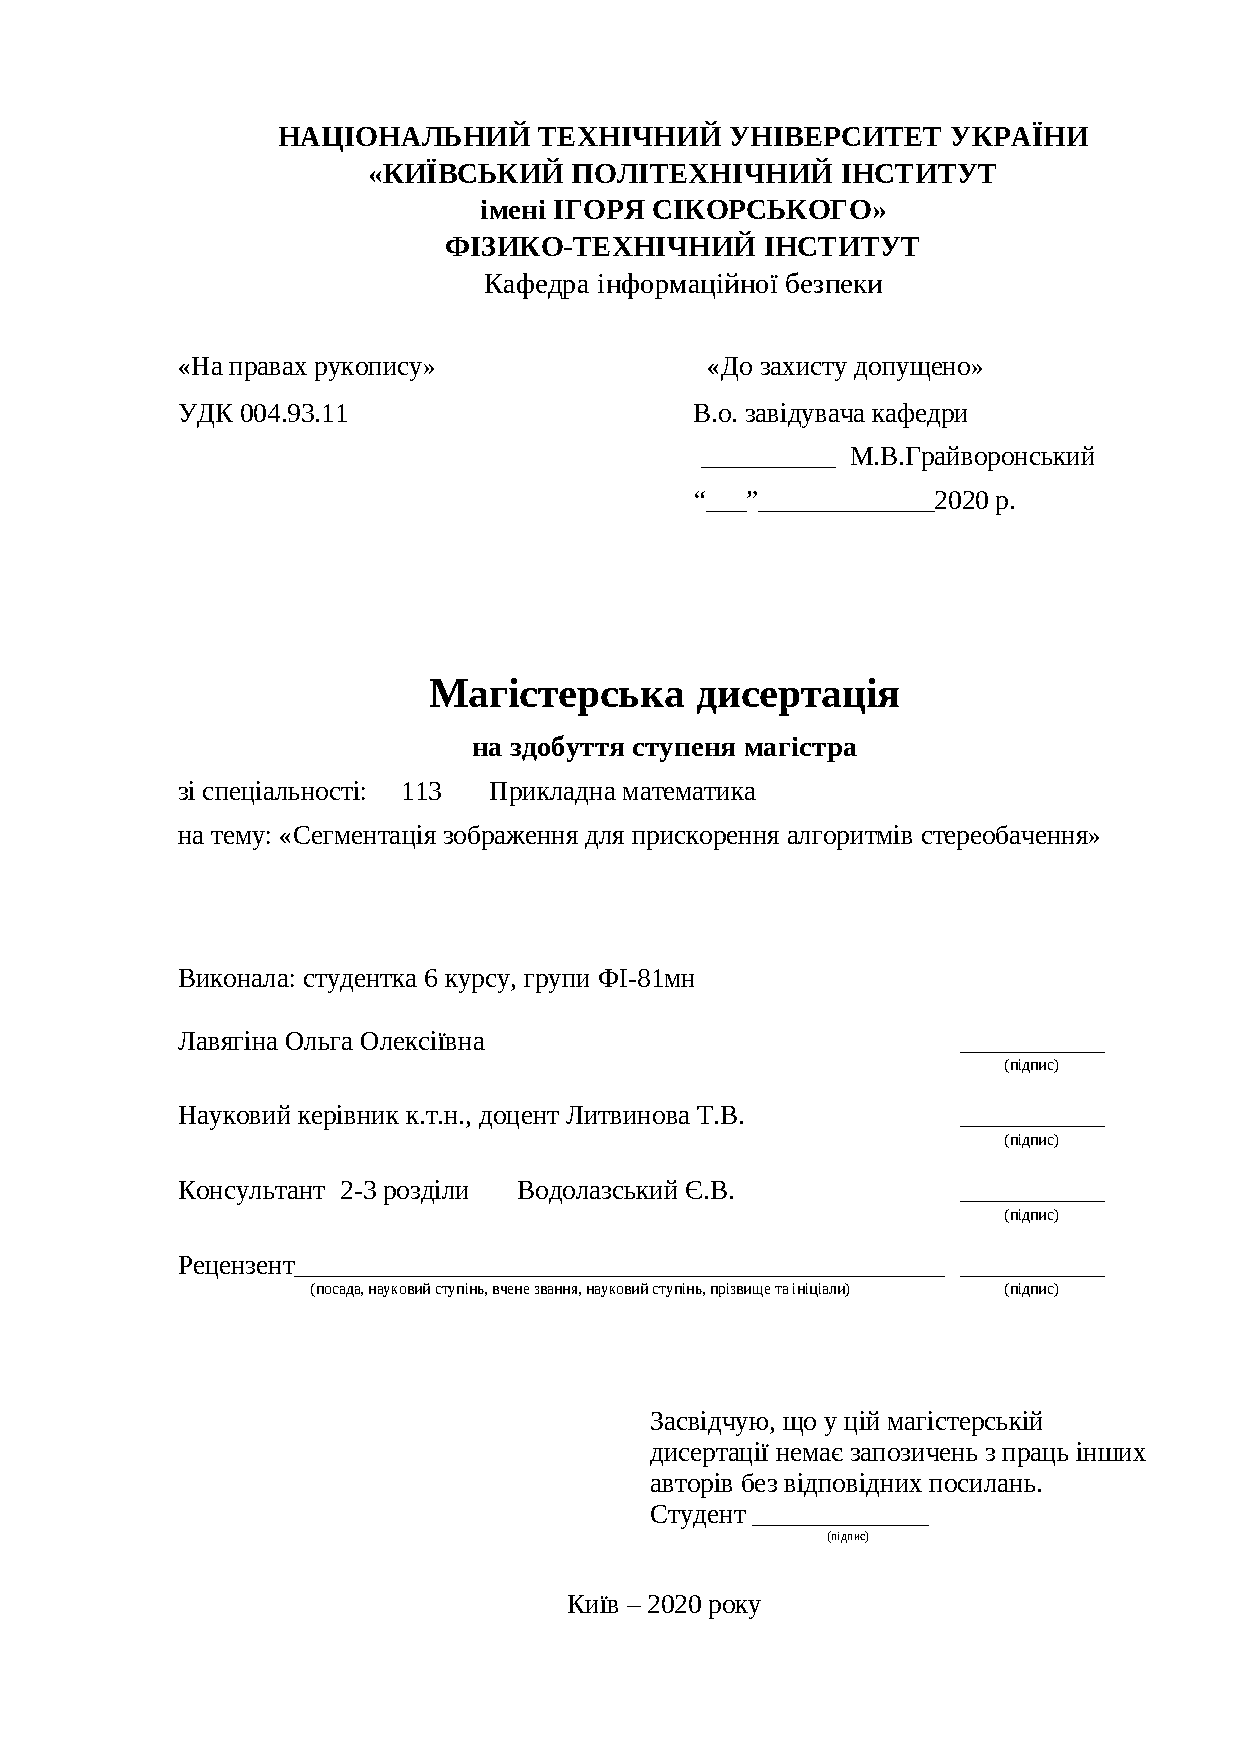
\includepdf[page=-]{title_filled}
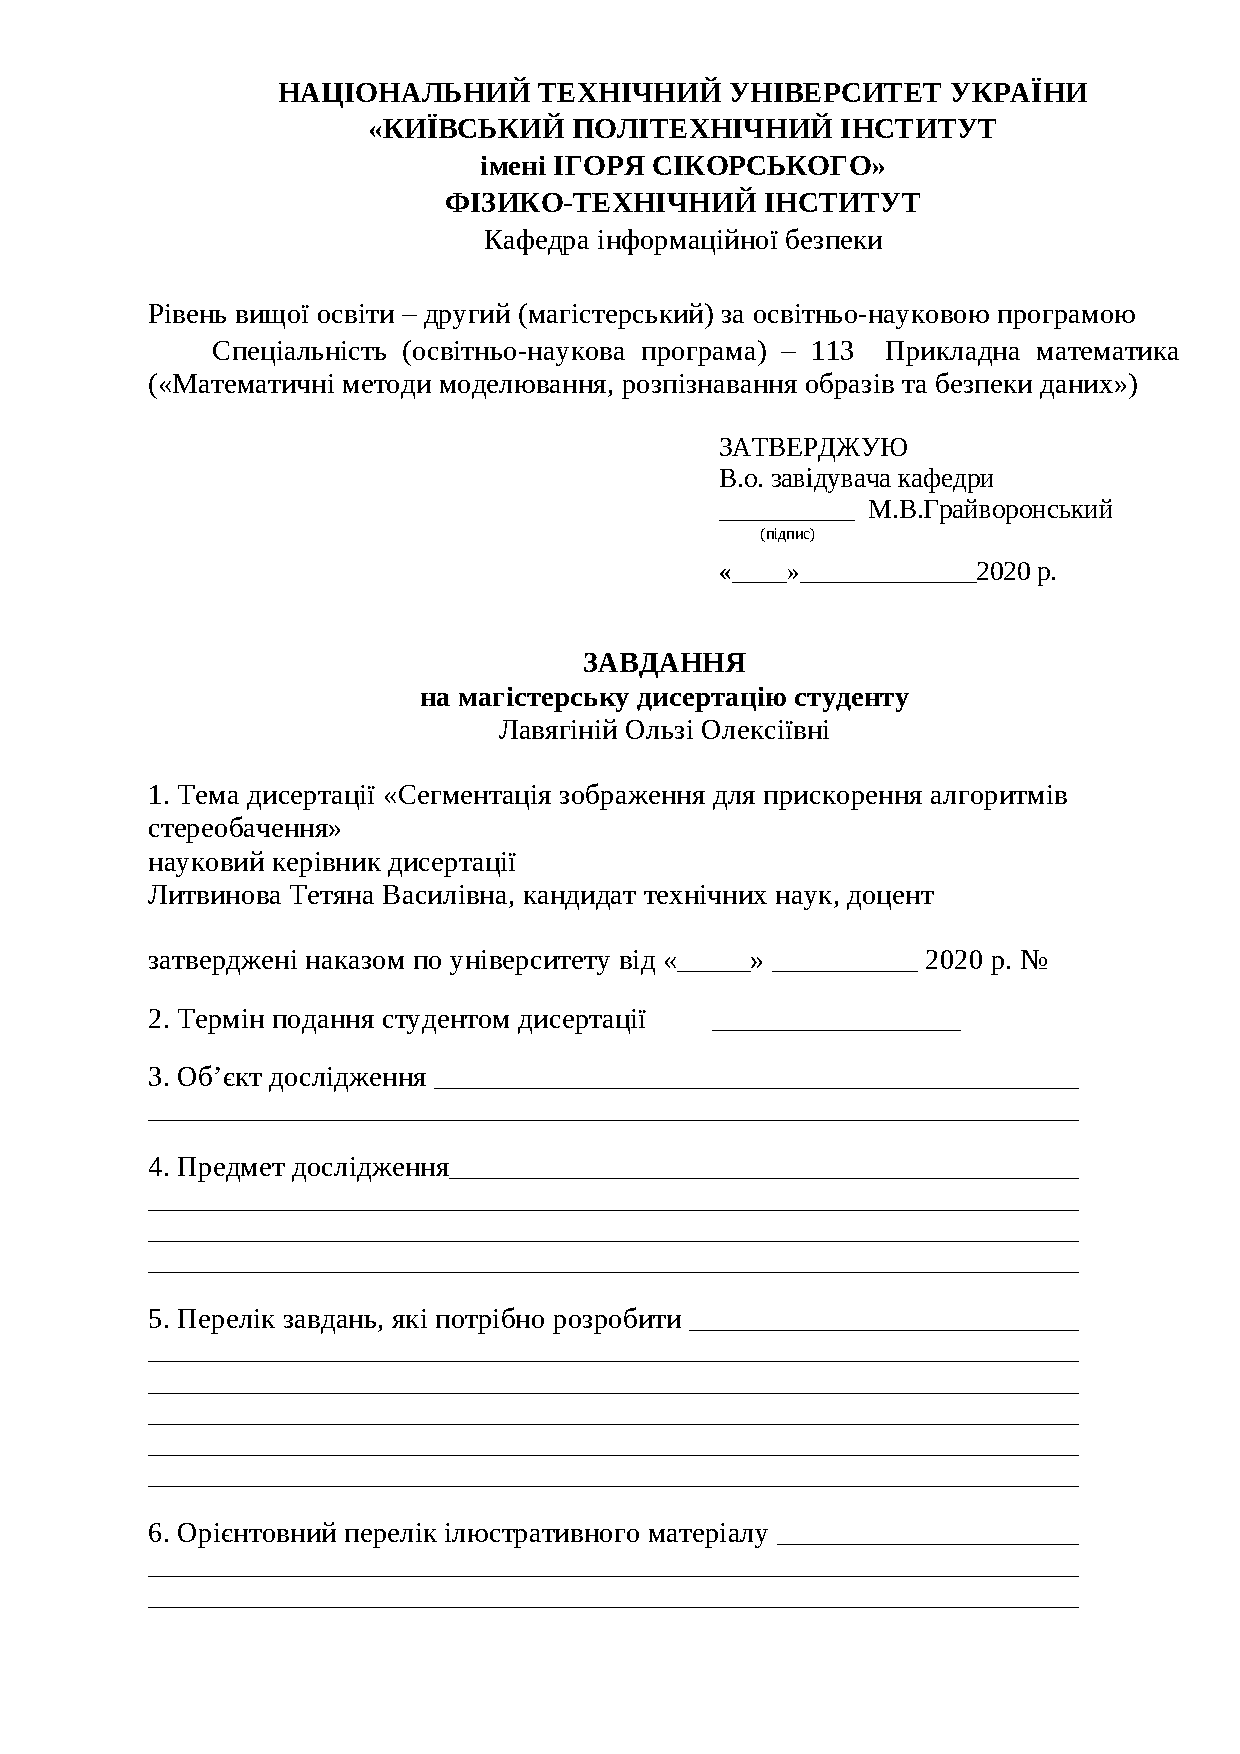
\includepdf[page=-]{task}

\clearpage
\pagenumbering{gobble}
\import{abstract/}{main.tex}

\tableofcontents

\clearpage
\pagenumbering{arabic}
\pagestyle{fancy}
\setcounter{page}{8}

\clearpage

% TODO: Add "theorem", "statement", "definition", bold or italic font

\import{preface/}{preface.tex}
\import{main/}{problem.tex}
\import{main/}{diffusion.tex}
\import{main/}{segmentation.tex}
\import{main/}{results.tex}

\import{conclusion/}{conclusion.tex}

\clearpage
\phantomsection
\addcontentsline{toc}{chapter}{Перелік посилань}
\renewcommand\bibname{Перелік посилань}
\bibliography{bibliography.bib}

\end{document}
